\documentclass[conference]{IEEEtran}
\IEEEoverridecommandlockouts
% The preceding line is only needed to identify funding in the first footnote. If that is unneeded, please comment it out.
\usepackage{cite}
\usepackage{amsmath,amssymb,amsfonts}
\usepackage{algorithmic}
\usepackage{graphicx}
\usepackage{textcomp}
\usepackage{xcolor}
\usepackage{url}
\usepackage{hyperref}
\usepackage{float}
\usepackage{moresize}
\usepackage{booktabs}


\makeatletter
\newcommand{\linebreakand}{%
  \end{@IEEEauthorhalign}
  \hfill\mbox{}\par
  \mbox{}\hfill\begin{@IEEEauthorhalign}
}
\makeatother



\def\BibTeX{{\rm B\kern-.05em{\sc i\kern-.025em b}\kern-.08em
    T\kern-.1667em\lower.7ex\hbox{E}\kern-.125emX}}
\begin{document}

\title{¿Quién gasta más y quién se registra? Evidencia observacional en CheMarket}

\author{%
\IEEEauthorblockN{Adrián Arturo Suárez García}
\IEEEauthorblockA{202123771\\
\href{mailto:a.suarezg@uniandes.edu.co}{\texttt{a.suarezg@uniandes.edu.co}}}
\and
\IEEEauthorblockN{Luis Alejandro Rubiano Guerrero}
\IEEEauthorblockA{202013482\\
\href{mailto:la.rubiano@uniandes.edu.co}{\texttt{la.rubiano@uniandes.edu.co}}}
\and
\IEEEauthorblockN{Gabriel Alejandro Moreno Riveros}
\IEEEauthorblockA{202014583\\
\href{mailto:g.morenor@uniandes.edu.co}{\texttt{g.morenor@uniandes.edu.co}}}
}



\maketitle


\section{Introducción}
A través de este informe, nuestro grupo de economistas y científicos de datos emplea diferentes técnicas de análisis estadístico y de machine learning para estudiar el comportamiento de los usuarios en \textbf{CheMarket Inc.} En particular, nos enfocamos en entender qué variables impulsan el revenue de la compañía, con el fin de generar evidencia que apoye la toma de decisiones estratégicas informadas.

El análisis se divide en dos partes complementarias. En la primera parte, trabajamos con datos observacionales para explorar patrones en el comportamiento de los usuarios: ¿quiénes gastan más?, ¿qué factores están asociados con el registro en la plataforma?, ¿qué variables ayudan a predecir el gasto individual? A partir de regresiones y modelos predictivos evaluamos si existe una diferencia sistemática en el gasto entre usuarios registrados y no registrados, y discutimos posibles sesgos que afectan la interpretación causal.

En la segunda parte, analizamos un experimento aleatorio en el que se facilitó el proceso de registro para un grupo de usuarios. Esta intervención nos permite estimar de manera más rigurosa el efecto del registro sobre el gasto, así como evaluar la efectividad del nuevo diseño en incrementar la tasa de registros. Finalmente, reflexionamos sobre la validez de los resultados, las limitaciones del experimento y presentamos recomendaciones concretas sobre si conviene escalar esta intervención.

En particular, encontramos que si bien existe una correlación entre registro y el aumento del gasto de los usuarios, no se puede inferir causalidad a partir de esta relación, ya que hay factores, tanto observables como no observables que están afectando directamente el ingreso, o de manera indirecta a través de la probabilidad de registro. Asimismo, consideramos que una interfaz más rápida para el registro aumenta la probabilidad de registro y el gasto de los usuarios, sin embargo, se debe ser cuidadosos con estos hallazgos ya que hay separación perfecta al estimar el registro en función de la interfaz,
 lo que puede hacer invalido extrapolar estos hallazgos, y sugiere un problema de diseño del experimento. Nuestra recomendación en particular es de no escalar este experimento.

\section{Datos observacionales: ¿Qué impulsa las ventas?}

\subsection{Datos y preparación}

Para el análisis observacional, contamos con un conjunto de $100.000$ observaciones históricas de los usuarios de CheMarket. Las variables disponibles son $\texttt{time\_spent}$: tiempo en el sitio durante la sesión, $\texttt{past\_sessions}$: número de sesiones anteriores, 
$\texttt{device\_type}$: tipo de dispositivo (móvil, escritorio, tablet), $\texttt{os\_type}$: sistema operativo (OS X, Windows, otros), $\texttt{is\_returning\_user}$: si el usuario ya había visitado antes, $\texttt{sign\_up}$: si se registró o no y $\texttt{revenue}$: cuanto gastó en cada sesión.

En la siguiente tabla se presentan las estadísticas descriptivas de estas variables.


\begin{table}[H]
\ssmall
\centering
\caption{Estadísticas descriptivas de las variables}
\begin{tabular}{|l|c|c|c|c|c|c|}
\hline
 & \textbf{Tiempo} & \textbf{Sesiones} & \textbf{Dispositivo} & \textbf{OS} & \textbf{Recurrente?} & \textbf{Revenue} \\
\hline
Mín & 0.000125 & 0 & Tablet: 9882 & Otro: 9909 & No: 4930 & 0.5451 \\
25\% & 1.4247 & 2 & Escritorio: 40009 & OS X: 30253 & Sí: 95070 & 2.3400 \\
Mediana & 3.4384 & 3 & Móvil: 50109 & Windows: 59838 & & 3.1370 \\
50\% & 4.9946 & 3.001 & & & & 3.9766 \\
75\%  & 6.9117 & 4  & & & & 4.5221 \\
Máx & 54.3989 & 14  & & & & 36.2934 \\
\hline
\end{tabular}

\hfill \break
Estadísticas descriptivas de las variables numéricas y cantidad por clase para las categóricas.

\end{table}

En la siguiente figura se presentan las distribuciones originales de \texttt{Revenue} y \texttt{time\_spent}.
Se puede observar que la densidad de ambas variables muestra muchos valores pequeños y pocos muy grandes.
Para nuestro análisis decidimos aplicar una transformación logarítmica y de raíz cuadrada respectivamente,
ya que estas transformaciones comprimen la cola y acercan la distribución a algo más gaussiano, 
lo que beneficia métodos lineales y tests que asumen normalidad de errores.


\begin{figure}[H]
    \centering
    \includegraphics[width=0.3\textwidth]{figures/revenueA.png}

    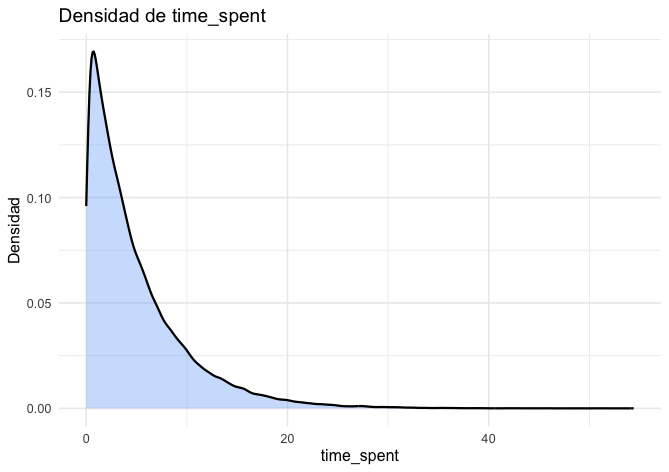
\includegraphics[width=0.3\textwidth]{figures/timespentA.png}
    \caption{Distribución de \texttt{Revenue} y \texttt{time\_spent}}
    \label{fig:distribucion}
\end{figure}



\subsection{Estimación del efecto de registrarse sobre el gasto}

En este caso queremos analizar el efecto de registrarse sobre el gasto de los usuarios. 
Sin embargo, es importante tener en cuenta que la relación entre estas variables puede estar influenciada por otras variables de nuestro modelo, 
en particular, en el siguiente gráfico presentamos como cambia el gasto dentro de diferentes clases de usuarios.

\begin{figure}[H]
    \centering
    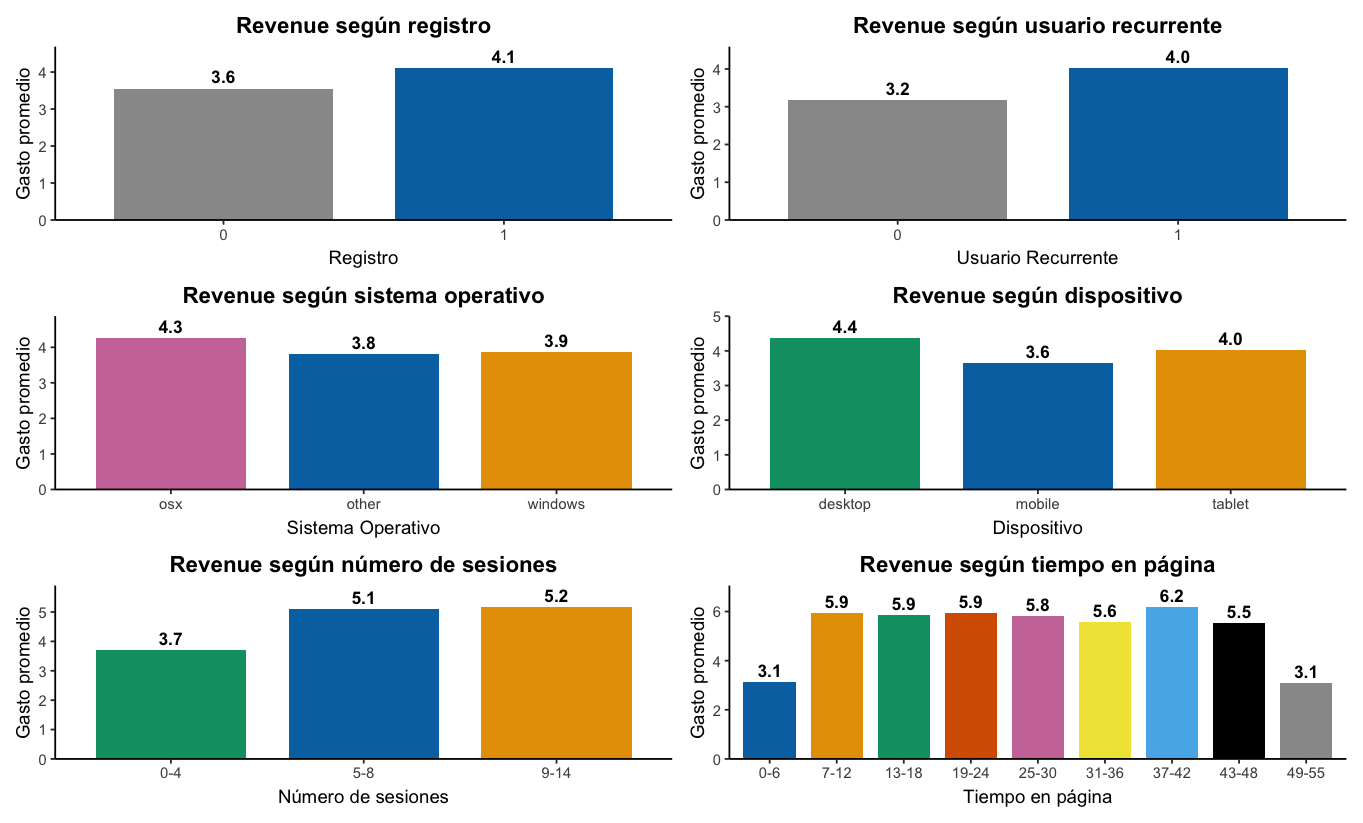
\includegraphics[width=0.5\textwidth]{figures/GastoA.png}
    \caption{Gasto promedio por clase de usuario}
    \label{fig:coefplot}
\end{figure}

Queremos tener esto en cuenta ya que estimar de manera ingenua el efecto del registro sobre el gasto podría llevar a conclusiones erróneas.
Por ejemplo, si observamos que los usuarios registrados tienden a gastar más, esto podría deberse a que otras variables los hicieron registrarse, y puede que estas variables también
estén teniendo un efecto sobre el gasto.


Teniendo conocimiento de nuestro datos pasamos a estimar el efecto promedio del registro de los usuarios sobre el ingreso total de la compañía, 
para esto usamos diferentes métodos de machine learning. La primera estimación consiste en estimar el efecto promedio puro sin incluir variables de control, en la segunda incluimos las variables pertinentes considerando
 la posible correlación que exista entre estas y el ingreso, o también entre estas y el registro.

 \begin{align*}
\textbf{M1:} \quad \log(\text{ingreso}) 
  &= \beta_{0} + \beta_{1}\,\text{registro} + \varepsilon \\[1em]
\textbf{M2:} \quad \log(\text{ingreso}) 
  &= \beta_{0} + \beta_{1}\,\text{registro} \\
     &+ \beta_{2}\,\sqrt{\text{tiempo en página}}\\
     &+ \beta_{3}\,\text{número de sesiones} \\
  &\quad + \beta_{4}\,\text{tipo dispositivo}\\
     &+ \beta_{5}\,\text{usuario recurrente}\\
     &+ \beta_{6}\,\text{sistema operativo}\\
     &+ \varepsilon \\
\end{align*}

\begin{table}[H]
\ssmall
\centering
\begin{tabular}{l c c}
\hline
\textbf{Variable} & \textbf{Coeficiente estimado M2} & \textbf{Coeficiente estimado M1} \\
\hline
Intercepto                 & 0.577  & 1.1405 \\
Registro (sign\_up = 1)     & 0.034 & 0.102 \\
Raíz cuadrada del tiempo en sitio & 0.241 &  \\
Sesiones pasadas            & 0.078 & \\
Dispositivo: Escritorio     & 0.081 & \\
Dispositivo: Móvil          & -0.102 & \\
Usuario recurrente          & -0.103 & \\
Sistema Operativo: OSX      & 0.049 & \\
Sistema Operativo: Windows  & 0.009 & \\
\hline
\end{tabular}

\hfill \break
Coeficientes estimados del modelo lineal para \texttt{log(Revenue)}
\end{table}




Es importante mencionar que en estas estimaciones se usa como base del modelo “tablet” para tipo dispositivo 
y “otro” para tipo sistema operativo.
 
Al estimar el primer modelo encontramos que, en promedio, el aumento de una unidad de registro incrementa en un $0.102$
 el logaritmo del ingreso para la compañía. Esto implica un aumento bastante significativo. No obstante, cuando, controlamos por las demás variables, este aumento promedio pasa a ser $0.034$, mucho menor, aproximadamente de de  $3.5$ puntos porcentuales en el revenue. Esto claramente indica que si existe una correlación entre el registro de los usuarios y su gasto, pero no necesariamente una causalidad, dado que el efecto es muy débil. Continuando con nuestra investigación, encontramos que casi el $80\%$ de los usuarios está registrado, y entendemos que un negocio de venta en línea requiere que las personas registren sus datos para enviar los productos, 
 además de implicar que gasten tiempo en la página. Por esto, existen variables omitidas respecto a la verdadera intención de gastar. No se gasta más por registrarte, el usuario se registra porque tiene intención de gastar. De hecho, también se observa una diferencia de 0,4 puntos más en gasto promedio si la persona emplea un sistema operativo de Apple, lo cual da indicios de una fuerte variable omitida, el ingreso. Si la persona tiene un celular alta gama, su ingreso puede ser mayor, por lo cuál gasta más, y se registra para gastar.

 Con esto en mente, desarrollamos un modelo para estimar qué variables afectan más el registro de los usuarios. El punto clave es buscar profundizar en nuestro informe para mejorar la comprensión del negocio respecto a su página web,
 
 si hay alta correlación entre el registro y el gasto, podemos ver qué variables afectan directamente el gasto y cuales lo hacen mediante el registro. Así, estimamos el modelo: 


\[
\Pr(\text{registro} = 1 \mid X) \;=\; \frac{\exp(X\beta)}{1 + \exp(X\beta)}
\]

con
\begin{align*}
    X\beta & = \beta_0 \\
    & + \beta_1 \sqrt{\text{tiempo en página}} \\
    & + \beta_2 \,\text{número de sesiones} \\
    & + \beta_3 \,\text{tipo dispositivo} \\
    & + \beta_4 \,\text{usuario recurrente} \\
    & + \beta_5 \,\text{ sistema operativo} \\
    & + \varepsilon.
\end{align*}

\begin{table}[H]
\centering
\begin{tabular}{l c}
\hline
\textbf{Variable} & \textbf{Coeficiente} \\
\hline
Intercepto             & 1.183951 \\
Sesiones pasadas       & 1.133554 \\
Dispositivo: Escritorio & 0.957080 \\
Dispositivo: Móvil      & 1.106124 \\
Sistema Operativo: OSX  & 1.077781 \\
Sistema Operativo: Windows & 1.021961 \\
Usuario recurrente      & 1.321484 \\
Raíz cuadrada del tiempo en sitio & 1.199510 \\
\hline
\end{tabular}

\hfill \break

Coeficientes estimados del modelo logístico para \texttt{sign\_up}

\end{table}

Los resultados de este modelo confirman nuestra hipótesis. Concretamente, se encontró que la probabilidad de registro aumenta $32$\% si la persona ha entrado previamente (por cada sesión pasada, la probabilidad de registro aumenta $13$\% en promedio), así como por cada minuto extra en la aplicación aumenta en promedio hasta $20$\% la probabilidad de registro. Esto nos dice que el registro está fuertemente influenciado por cuánto tiempo pasan las personas en la aplicación y cuántas veces han vuelto; es decir, si una persona es recurrente, si pasa mucho tiempo en la app, seguramente se registra para poder comprar. 


\subsection{Capacidad predictiva del modelo}

Para analizar la capacidad predictiva del modelo, dividimos nuestro dataset en un conjunto de entrenamiento y otro de validación, usando un split $70/30$, y la semilla $2025$ para asegurar la reproducibilidad.

Para esto, conociendo las interacciones de nuestras variables respecto al gasto de los usuarios, desarrollamos diversos modelos predictivos. El objetivo de desarrollar varios modelos es buscar la complejidad ideal de balance entre sesgo y varianza, es decir, que relacione las variables tal que se ajuste bien a los datos, pero no adopte completamente el ruido blanco de la muestra.

\begin{align*}
\textbf{M1 (básico):}\quad &\\
\log(\text{ingreso}) \;=\;& \; \beta_0 \nonumber \\
&+ \beta_1 \,\text{registro} \nonumber \\
&+ \varepsilon \\[1em]
%
\textbf{M2 (controles):}\quad &\\
\log(\text{ingreso}) \;=\;& \; \beta_0 \nonumber \\
&+ \beta_1 \,\text{registro} \nonumber \\
&+ \beta_2 \,\sqrt{\text{tiempo en página}} \nonumber \\
&+ \beta_3 \,\text{número de sesiones} \nonumber \\
&+ \beta_4 \,\text{tipo dispositivo} \nonumber \\
&+ \beta_5 \,\text{usuario recurrente} \nonumber \\
&+ \beta_6 \,\text{sistema operativo} \nonumber \\
&+ \varepsilon \\[1em]
%
\textbf{M3 (interacciones):}\quad &\\
\log(\text{ingreso}) \;=\;& \; \beta_0 \nonumber \\
&+ \beta_1 \,\text{registro} \nonumber \\
&+ \beta_2 \,\sqrt{\text{tiempo en página}} \nonumber \\
&+ \beta_3 \,\text{número de sesiones} \nonumber \\
&+ \beta_4 \,\text{tipo dispositivo} \nonumber \\
&+ \beta_5 \,\text{usuario recurrente} \nonumber \\
&+ \beta_6 \,\text{sistema operativo} \nonumber \\
&+ \beta_7 \,(\text{registro} \times \text{número de sesiones}) \nonumber \\
&+ \beta_8 \,(\text{registro} \times \text{sistema operativo}) \nonumber \\
&+ \beta_9 \,(\text{registro} \times \text{tipo dispositivo}) \nonumber \\
&+ \beta_{10} \,(\text{registro} \times \text{usuario recurrente}) \nonumber \\
&+ \varepsilon
\end{align*}

Validamos la capacidad de predicción de nuestros modelos calculando el cuadrado del error, 
que es una medida de la diferencia promedio entre la predicción del modelo y el valor real. 
Los resultados fueron: $0.2839$, $0.1984$ y $0.1982$. Esto nos indica que al inducir los controles minimizamos el error, es decir,
 nuestra predicción mejora, pero inducir complejidad mediante interacciones ya no mejora significativamente. 
 Incluso se introdujeron relaciones cuadráticas y no tuvo efecto alguno. 


\subsection{Recomendación preliminar}


Basados en los hallazgos anteriores, la evidencia estadística en este informe muestra que no existen indicios de causalidad 
entre el registro y el gasto de cada usuario, por lo que no recomendamos realizar un experimento para confirmarla. Consideramos que hay variables omitidas, como el salario de los usuarios, o el tiempo que pasan en la aplicación, que son más efectivos para aumentar el ingreso. 
Invertir en programas de marketing que se enfoquen en audiencias específicas, o diseñar la página para aumentar la retención de los usuarios, registrados o no, son usos más efectivos de los recursos de la compañía.



\section{Datos experimentales: ¿Funciona facilitar el registro?}

\subsection{Verificación del experimento}

Se implementó un cambio en el diseño del sitio para facilitar el proceso de registro. 
Esta intervención fue asignada aleatoriamente a algunos usuarios, lo que permite evaluar su impacto sobre el gasto 
como un experimento de manera más rigurosa.

Queremos ver si el experimento fue bien implementado, es decir, si los grupos de control y tratamiento son comparables en términos de características observables.

Para ello, se realizó un análisis de balance entre el grupo de tratamiento y el de control. Para las variables continuas se aplicaron pruebas $t$ de diferencias de medias, mientras que para las categóricas se emplearon pruebas de Chi-cuadrado ($\chi^2$), además de comprobar de manera gráfica.
En la siguiente figura se muestran las medias de las diferentes covariables entre los grupos de tratamiento y control. Posteriormente, se muestran los resultados 
estadísticos de la prueba de diferencia de medias.

\begin{figure}
    \centering
    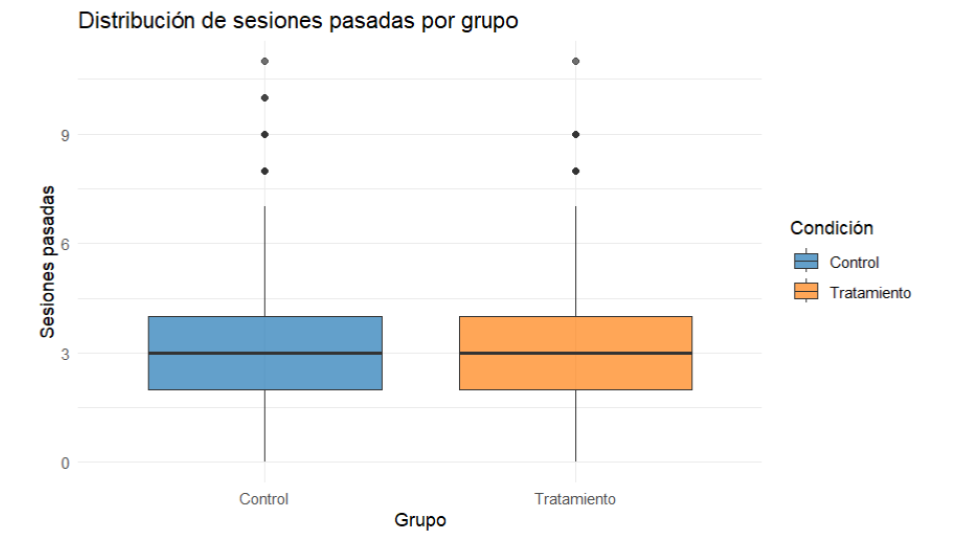
\includegraphics[width=0.3\textwidth]{figures/21.png}

    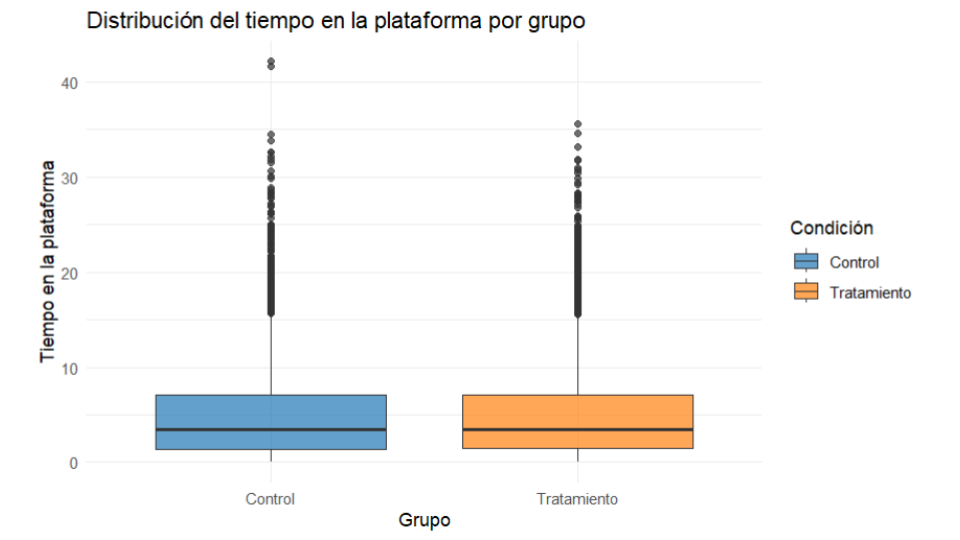
\includegraphics[width=0.3\textwidth]{figures/22.png}

    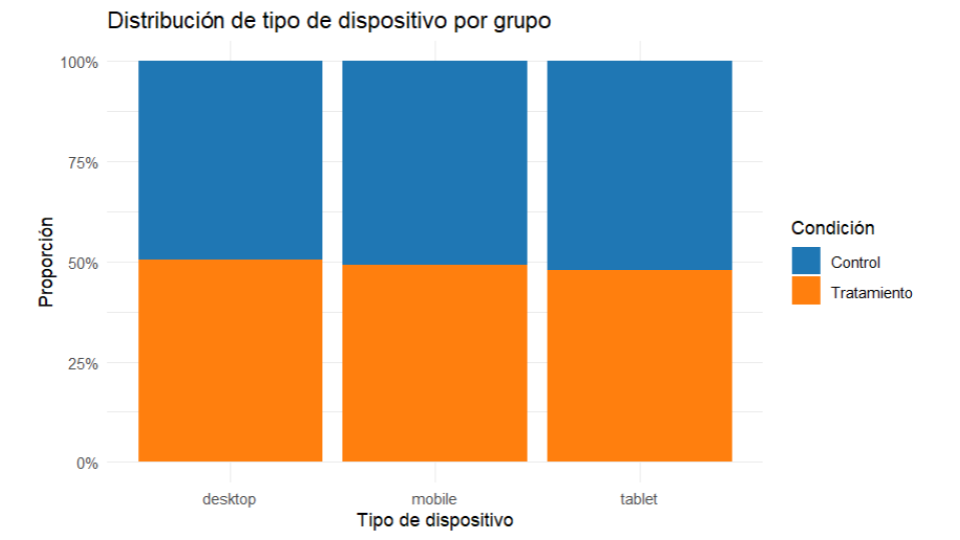
\includegraphics[width=0.3\textwidth]{figures/23.png}

    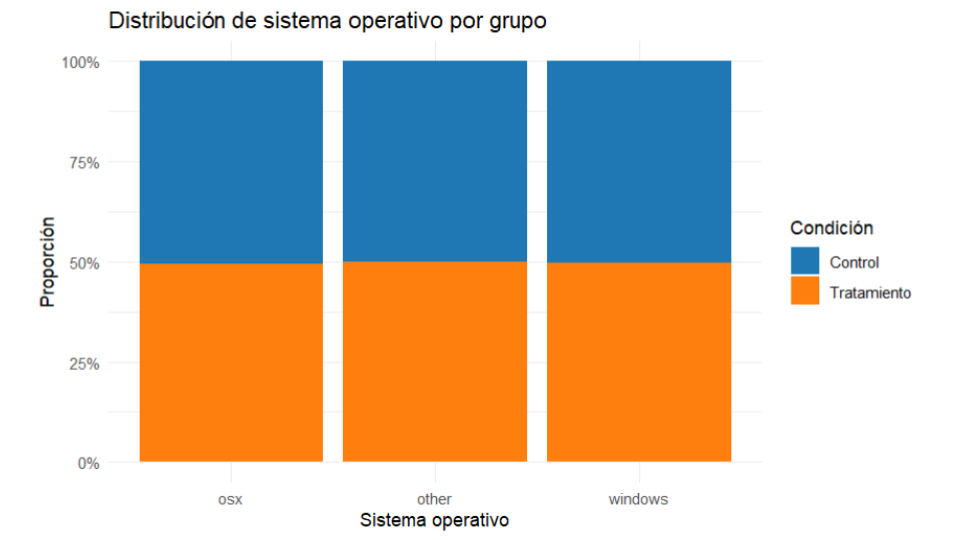
\includegraphics[width=0.3\textwidth]{figures/24.png}

    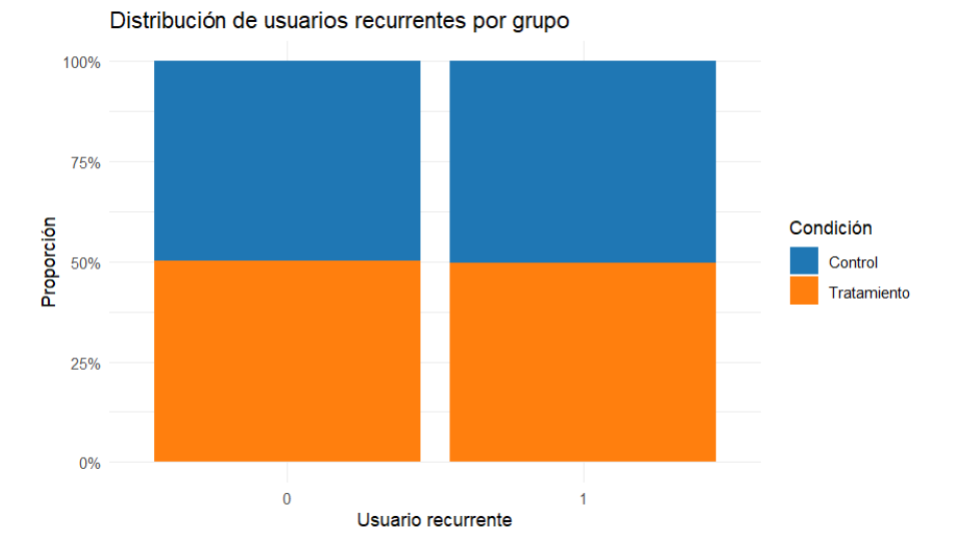
\includegraphics[width=0.3\textwidth]{figures/25.png}


    \caption{Análisis de balance entre grupos de tratamiento y control}
    \label{fig:balance}
\end{figure}

\begin{table}[H]
\ssmall
\centering
\caption{Balance entre grupos de control y tratamiento}
\label{tab:balance}
\begin{tabular}{lccc}
\hline
\textbf{Variable} & \textbf{Media (Control)} & \textbf{Media (Tratamiento)} & \textbf{p-valor (test)} \\ 
\hline
Tiempo en plataforma & 4.97 & 5.09 & 0.247 \\
Sesiones pasadas     & 2.99 & 3.04 & 0.245 \\
Tipo de dispositivo  & --   & --   & 0.210 (Chi$^2$) \\
Sistema operativo    & --   & --   & 0.924 (Chi$^2$) \\
Usuario recurrente   & --   & --   & 0.771 (Chi$^2$) \\
\hline
\end{tabular}

\hfill \break
Prueba de balance entre grupos de control y tratamiento. 
\end{table}

Los resultados muestran que no existen diferencias estadísticamente significativas entre los grupos en las covariables observadas. Esto respalda la validez del procedimiento de asignación aleatoria, garantizando que el tratamiento y el control son comparables al inicio del experimento.


\subsection{Efecto sobre el registro}

Con el objetivo de evaluar si una interfaz más rápida en el proceso de registro incrementa la probabilidad de que los usuarios completen exitosamente su inscripción en la plataforma,
se estimó un modelo de regresión logística para identificar el efecto del tratamiento sobre la probabilidad de registro, los resultados se presentan en la siguiente tabla.

\begin{table}[H]
\centering
\caption{Efecto del tratamiento sobre el registro}
\label{tab:glm_signup_treatment}
\begin{tabular}{lcc}
\toprule
 & \textbf{Coeficiente} & \textbf{Error estándar} \\ 
\midrule
Intercepto & -3.06e-14*** & (4.35e-16) \\
Tratamiento (easier\_signup) & 1.000*** & (6.17e-16) \\
\midrule
Observaciones & \multicolumn{2}{c}{10,000} \\
\bottomrule
\multicolumn{3}{l}{Errores estándar entre paréntesis.} \\
\multicolumn{3}{l}{$*** p < 0.01, ** p < 0.05, * p < 0.1$.} \\
\end{tabular}

\hfill \break

Regresión logística para estimar el efecto del tratamiento sobre la probabilidad de registro.
\end{table}

Los resultados muestran que crear una interfaz de rápido acceso hace que prácticamente todos los individuos del grupo de tratamiento completaron el registro, en contraste con el grupo de control. Sin embargo, la magnitud absoluta del efecto (100\%) sugiere la presencia de separación perfecta, lo que obliga a ser prudentes en la generalización a otros contextos.


\subsection{Efecto sobre el gasto}

Con el objetivo de evaluar si una interfaz más rápida en el proceso de registro incrementa la gasten en la plataforma, se estimó un modelo de regresión para identificar el efecto del tratamiento sobre la ganancias. Los resultados se presentan en la siguiente tabla.

\begin{table}[H]
\centering
\caption{Efecto del tratamiento sobre los ingresos}
\begin{tabular}{lcc}
\toprule
 & \textbf{Coeficiente} & \textbf{Error estándar} \\ 
\midrule
Intercepto & 3.978*** & (0.051) \\
Tratamiento (easier\_signup) & 0.491*** & (0.073) \\
\midrule
Observaciones & \multicolumn{2}{c}{10,000} \\
R-cuadrado & \multicolumn{2}{c}{0.0045} \\
\bottomrule
\multicolumn{3}{l}{Errores estándar entre paréntesis.} \\
\multicolumn{3}{l}{$*** p < 0.01, ** p < 0.05, * p < 0.1$.} \\
\end{tabular}
\end{table}

Los resultados muestran que las personas que usan una interfaz mas rapida generaron $0.49$ unidades monetarias más de ingreso que las personas con la interfaz original, sin embargo este efecto no es significativo sólo explica una pequeña parte de la variación de los ingresos por $R^2 (0.0045)$. 



\subsection{Limitaciones y robustez}

El experimento aleatorio proporciona evidencia clara de que la interfaz más rápida aumenta los registros y produce un incremento promedio en ingresos. Sin embargo hay problemas con la separación perfecta entre tratados y controles, lo que puede implicar que la magnitud del experimento no sea totalmente fiable. La presencia potencial de variables omitidas podría explicar la separación perfecta además de sesgar la estimación. Otra limitación del experimento es el bajo poder explicativo que tiene el experimento ya que la mayor parte de la variación en Revenue queda sin explicar, lo que sugiere heterogeneidad relevante entre usuarios y limita la capacidad del experimento para predecir resultados económicos agregados.




\subsection{Recomendación final}


El experimento muestra que la interfaz de registro más rápida genera un efecto positivo tanto en los ingresos como en la tasa de registros. Sin embargo, recomendamos mantener la intervención en la escala actual antes de una expansión, dado que la base de información disponible es limitada y puede ocultar factores relevantes que influyen en la relación observada, lo que introduce un riesgo de sesgo por omisión. Para reducir esa incertidumbre y mejorar la capacidad explicativa del modelo, es necesario ampliar la recolección de datos incorporando variables adicionales sobre el comportamiento de los usuarios, características de perfil, factores contextuales. de modo que el análisis econométrico pueda ofrecer estimaciones más sólidas y confiables que sustentan una decisión estratégica con mayor certeza.





\section{Conclusiones}


En conjunto, la evidencia observacional y experimental sugiere que el registro está asociado con mayores ingresos, pero el vínculo causal es débil y sensible a la especificación del modelo. Más bien, el registro parece actuar como marcador de intención de compra, impulsado por variables como el tiempo en página y el número de sesiones previas. El experimento de “registro más fácil” incrementó sustancialmente la tasa de registros y mostró un efecto promedio positivo sobre los ingresos, aunque con poder explicativo muy bajo y señales de separación perfecta que obligan a interpretar con cautela la magnitud del impacto. Recomendamos no escalar la intervención de forma masiva por ahora y mantenerla en el alcance actual mientras se corrigen limitaciones: (i) rediseñar el experimento para evitar separación, (ii) ampliar la recolección de covariables relevantes (canal de adquisición, ubicación, proxies de ingreso), y (iii) evaluar impacto económico neto con métricas de negocio (retención, costos marginales, etc). Con estos ajustes, futuros experimentos podrán ofrecer estimaciones más robustas y útiles para una decisión estratégica de escalamiento.


\end{document}
